% ==============================================================================
% NeurIPS 2026 Main Conference Paper — 9 pages + references
% Main paper file — includes result tables via \input
% ==============================================================================

\documentclass{article}

% Anonymous submission (double-blind for Main Track)
\usepackage{neurips_2026}

% ---------- Packages ----------
\usepackage[utf8]{inputenc}
\usepackage[T1]{fontenc}
\usepackage{amsmath,amssymb,amsfonts}
\usepackage{graphicx}
\usepackage{booktabs}
\usepackage{enumitem}
\usepackage{hyperref}
\usepackage{url}
\usepackage{xcolor}
% natbib loaded by neurips_2026.sty — do not reload
\usepackage{microtype}

% ---------- Custom commands ----------
\newcommand{\sone}{S1-like}
\newcommand{\stwo}{S2-like}
\newcommand{\pzero}{\texttt{P0}}
% ---------- Title ----------
\title{Readable but Not Writable: Reasoning Training Decouples\\
  Bias Directions from Behavior in LLMs}

\author{%
  \textbf{Anonymous Authors}\\
  Anonymous Institution\\
}

\date{}

\begin{document}

\maketitle

% ============================================================
% Abstract
% ============================================================

\begin{abstract}
Activation steering is a leading technique for controlling LLM behavior,
but we show it fails in reasoning-trained models.  Cognitive-bias
directions in activation space are \emph{readable but not writable}
after reasoning training: linearly decodable by probes, yet causally
inert under steering.
We compare matched-architecture pairs (Llama-3.1-8B-Instruct vs.\
R1-Distill-Llama-8B, OLMo-3 7B/32B Instruct vs.\ Think) and
Qwen-3-8B's thinking toggle, across 470 contrastive items spanning 11
bias categories (base-rate neglect, conjunction fallacy, framing, and
others).  Reasoning training collapses lure rates: 27.3\% to 2.4\%
(Llama), 19.6\% to 0.4\% at 32B.
Three results establish the dissociation.  First, probe-direction
steering on the three vulnerable categories produces a monotonic 37.5pp
dose-response in Llama (lure rates span 31\% at $\alpha$=+5 to 69\%
at $\alpha$=$-$5, zero incoherent outputs), while the same intervention
in R1-Distill, applied continuously across 2048 tokens at four layers
including its probe peak, produces no coherent shift.  Second,
Qwen-3-8B's think and no-think modes both achieve ${\sim}$0.97 probe
AUC yet cross-mode transfer is at chance (0.496), showing the decodable
direction is mode-specific.  Third, scaling to 32B amplifies
standard-model vulnerability (14.9\%$\to$19.6\%) while reasoning
training remains protective (0.4\% lure rate).
These results suggest that activation-steering safety interventions may
not transfer to reasoning models, and that reasoning training
reorganizes bias representations rather than layering deliberation atop
an unchanged substrate.
\end{abstract}

% ============================================================
% 1. Introduction (~1.5 pages)
% ============================================================

\section{Introduction}
\label{sec:intro}

Kahneman's dual-process framework distinguishes fast, heuristic
processing (``System~1'') from slow, deliberative processing
(``System~2'') \citep{kahneman2011thinking}.  While the binary framing
is an acknowledged oversimplification (modern accounts treat this as a
\emph{continuum} of processing intensity \citep{melnikoff2018mythical,
evans2013dual, deneys2023advancing}), the core observation that
cognitive systems flexibly allocate effort, with measurable consequences
for bias susceptibility, remains robust.  De~Neys' conflict
detection paradigm \citep{deneys2012bias, deneys2017dual} demonstrates
that humans often \emph{detect} conflicts between heuristic and
normative responses even when they fail to override the heuristic, a
dissociation between conflict \emph{monitoring} and conflict
\emph{resolution} with clear neural correlates in the anterior cingulate
cortex \citep{botvinick2001conflict}.

LLMs exhibit analogous patterns: instruction-tuned models reproduce
human-like errors on conflict items while succeeding on matched controls
\citep{hagendorff2023human}, and reasoning-trained models resist many
such lures \citep{deepseekr1}, though the protection is bias-specific
rather than universal \citep{schwartz2025clinical}.  A growing literature
documents these parallels \citep{codaforno2025dual,
ziabari2025reasoning}, and \citet{huang2026cogbias} showed that
bias-relevant directions are probeable and steerable.  We ask a
different question: what does reasoning post-training change about the
\emph{decodability}, layer location, and \emph{behavioral writability}
of those directions?

Yet behavior alone cannot distinguish genuine processing-mode differences
from surface mimicry: chain-of-thought traces are often unfaithful,
with only ${\sim}2.3$\% of reasoning steps causally influencing the
final answer \citep{jiang2025aha, lanham2023measuring,
boppana2026reasoning}.  The critical question is whether fast/slow modes
have \emph{mechanistic correlates} in internal representations, and how
those correlates change when a model is trained to reason.

Recent work on activation steering \citep{turner2023activation,
rimsky2024steering, cox2026decoding} has shown that targeted
interventions on internal representations modulate behavior causally,
with pre-CoT probes achieving $>$0.9 AUC and answer-flipping rates
above 50\% on instruction-tuned models \citep{cox2026decoding}.  This raises a
natural question for the dual-process setting: if linear probes identify
a direction in activation space that separates \sone{}-like from
\stwo{}-like processing, can steering along that direction
\emph{causally} modulate bias susceptibility?  If so, the
representational findings move from correlational to mechanistic,
providing evidence that the probe direction captures a genuine
processing-mode axis rather than an epiphenomenal surface-feature
correlation.

We address this question with a natural experiment: Llama-3.1-8B-Instruct
and DeepSeek-R1-Distill-Llama-8B share identical architectures (32
layers, 32 attention heads, 4096 hidden dimensions) but differ in
reasoning distillation training.  Representational differences are
thus primarily attributable to the post-training pipeline, not
architecture.  We make six contributions:

\begin{enumerate}[leftmargin=*,itemsep=2pt]
  \item A \textbf{contrastive cognitive bias benchmark} of 470 items
  (235 matched conflict/control pairs) across 11 categories spanning
  four heuristic families (representativeness, cognitive reflection,
  decision framing, and loss/availability), with novel isomorphs to resist
  memorization.

  \item \textbf{Behavioral validation} showing a large gap: 27.3\%
  overall lure rate (standard) vs.\ 2.4\% (reasoning), replicated on
  OLMo-3-7B (14.9\% $\to$ 0.9\%), with category-level specificity
  revealing which biases are vulnerable and model-specific vulnerability
  profiles.

  \item \textbf{Probing analysis} revealing that the standard model has
  high internal conflict/control separability (AUC\,=\,0.974) while the
  reasoning model renders this distinction \emph{less linearly accessible} (AUC\,=\,0.930),
  with cross-prediction and cross-model probe
  transfer (AUC\,$>$\,0.92) demonstrating specificity to a shared
  processing-mode direction.

  \item \textbf{Causal evidence via probe-direction steering and the \emph{readable but not writable} dissociation}: in Llama, steering along the probe weight vector produces a 37.5pp bidirectional causal swing, establishing the direction as causally active; in R1-Distill, the same direction is linearly decodable (AUC\,=\,0.930) but \emph{not stably controllable} at any of four layers (L14/L25/L28/L31) under continuous 2048-token intervention.

  \item \textbf{Within-CoT probing}: probe AUC follows a non-monotonic trajectory---peaking at onset (0.973), dropping during deliberation (0.754), rebounding before the answer (0.971)---indicating the trace is not representationally flat.

  \item \textbf{A training--inference dissociation}: Qwen~3-8B's think/no-think modes achieve similar conflict separability (AUC\,=\,0.954 and 0.970) but cross-mode probe transfer is at chance (AUC\,=\,0.496)---the two modes develop non-transferring conflict-encoding axes.
\end{enumerate}

\noindent We also analyze \textbf{scale effects} at 32B
(OLMo-3.1), finding that scale \emph{increases} standard-model
vulnerability while reasoning training remains protective, and report
converging SAE and attention entropy evidence.

% ============================================================
% 2. Related Work (~0.75 pages)
% ============================================================

\section{Related Work}
\label{sec:related}

\paragraph{Dual-process cognition in LLMs.}
\citet{hagendorff2023human} first documented human-like cognitive biases
in LLMs, finding that instruction-tuned models reproduce
representativeness and anchoring effects that vanish in later ChatGPT
versions.  \citet{codaforno2025dual} applied psychometric methods to show
that heuristic and deliberative prompts elicit shared early-layer
representations but diverge in later layers (a suggestive but purely
behavioral result).  \citet{ziabari2025reasoning} positioned reasoning
along a continuous spectrum rather than a binary, examining how reasoning
training shifts the balance between fast and slow processing modes.
\citet{brady2025dual} review the dual-process lens for LLM
decision-making in \emph{Nature Reviews Psychology}, noting that LLMs
mimic both System~1- and System~2-like responses but through mechanisms
distinct from human cognition.
Our work moves beyond behavioral characterization: we test whether the
System~1/System~2 distinction has a \emph{mechanistic} counterpart in
model internals.

\paragraph{Cognitive bias benchmarks and probing.}
\citet{malberg2025cognitive} surveyed 30 cognitive biases across 20 LLMs,
establishing that bias susceptibility varies systematically with model
scale and training recipe, but without examining internal representations.
Most directly relevant, \citet{huang2026cogbias} demonstrated that
cognitive bias directions are linearly decodable and steerable in LLM
residual streams, achieving 26--32\% bias reduction via contrastive
activation addition.  We differ from CogBias in three respects:
(i)~architecturally matched base--reasoning model pairs that isolate
reasoning training as the independent variable, (ii)~Hewitt--Liang
control tasks and cross-domain transfer tests as probe validity checks
\citep{hewitt2019control}, and (iii)~causal evidence via probe-direction
steering on a contrastive benchmark with matched conflict/no-conflict
items.

\paragraph{Activation steering and representation engineering.}
Activation addition \citep{turner2023activation} and its variants
\citep{rimsky2024steering, li2024inference} demonstrate that linear
steering vectors can modulate model behavior at inference time.
CogBias \citep{huang2026cogbias} applied this to cognitive bias (26--32\%
reduction), but used mean-difference vectors.  Our probe-direction
steering uses the probe's optimized weight vector, providing a tighter
causal link.  For SAE analysis, we adopt Ma et al.'s falsification
protocol \citep{ma2026falsification} as a mandatory filter, since
45--90\% of purported ``reasoning features'' are spurious token-level
artifacts \citep{meloux2025dead}.

\paragraph{Conflict detection in cognitive science.}
Our theoretical framework draws on De~Neys' conflict detection paradigm
\citep{deneys2012bias, deneys2017dual}, which demonstrates that humans
detect heuristic--normative conflicts even when they fail to override the
heuristic response.  \citet{evans2013dual} refined the Type~1/Type~2
taxonomy, emphasizing that the distinction is graded rather than binary,
a framing we adopt for LLMs.  \citet{botvinick2001conflict}'s conflict
monitoring theory provides the computational account: the anterior
cingulate cortex signals response conflict, triggering increased cognitive
control.  We test the LLM analogue of this account: do models show
internal signatures of conflict detection (elevated attention entropy,
reduced probe confidence) even when producing heuristic-driven responses?

% ============================================================
% 3. Benchmark (~0.5 pages)
% ============================================================

\section{Benchmark}
\label{sec:benchmark}

We construct a contrastive cognitive bias benchmark following three
design principles: (1) every conflict item has a structurally matched
no-conflict control \citep{deneys2012bias}; (2) all items use novel
surface features to resist memorization; and (3) category diversity
enables specificity analysis.

The benchmark comprises \textbf{470 items} organized as \textbf{235
matched pairs} across 11 categories spanning four heuristic families:
\emph{representativeness} (base rate neglect, 35 pairs; conjunction
fallacy, 20; belief-bias syllogisms, 25),
\emph{cognitive reflection} (CRT variants, 30; arithmetic, 25),
\emph{decision framing} (framing effects, 20; anchoring, 20), and
\emph{loss/availability} (sunk cost, loss aversion, certainty effect,
availability; 60 pairs total).  Base rate items include 10 pairs in
Gigerenzer's natural frequency format \citep{gigerenzer1995improve}.
Each item is scored as \emph{correct}, \emph{S1-lure} (the specific
heuristic-predicted wrong answer), \emph{other-wrong}, or \emph{refusal}.
Classic problems (e.g., the original bat-and-ball) serve only as
contamination baselines.

\paragraph{Item counts and analysis subsets.}
Our benchmark contains 470 items across 11 categories.  Primary probe
analyses use the 3 vulnerable categories (160 items).  Cross-prediction
uses all 7 original categories (350 items).  The full 11-category set
includes 4 additional categories added to test domain generality.

% ============================================================
% 4. Methods (~1 page)
% ============================================================

\section{Methods}
\label{sec:methods}

\subsection{Models}

Our headline comparison exploits the architectural identity between
\textbf{Llama-3.1-8B-Instruct} \citep{llama31} and
\textbf{R1-Distill-Llama-8B} \citep{deepseekr1}: both have 32
transformer layers, 32 query heads (8 KV heads via grouped-query
attention), and 4096 hidden dimensions.  The models differ primarily in that
R1-Distill-Llama-8B was distilled from a reasoning-trained teacher.  We
additionally evaluate \textbf{Qwen~3-8B} in both thinking (\texttt{/think})
and non-thinking (\texttt{/no\_think}) modes, providing a
\emph{within-model} toggle of reasoning behavior on identical weights.
For cross-architecture replication, we evaluate
\textbf{OLMo-3-7B-Instruct} and \textbf{OLMo-3-7B-Think}
\citep{olmo3}, which share the same OLMo base but differ in reasoning
training.  For scale analysis, we additionally evaluate
\textbf{OLMo-3.1-32B-Instruct} and \textbf{OLMo-3.1-32B-Think}
(64 layers, 4.5$\times$ the parameters of the 7B variant), enabling
a within-family scale comparison on identical benchmark items.

\paragraph{Prompting and decoding.}
All models use greedy decoding (\texttt{do\_sample=False}, \texttt{temperature=1.0})
with no system prompt. For Qwen~3-8B, we use the hard mode switch
(\texttt{enable\_thinking=True/False} in \texttt{apply\_chat\_template}).
In no-think mode, this appends an empty
\texttt{<think>{\textbackslash}n{\textbackslash}n</think>{\textbackslash}n{\textbackslash}n}
block after the assistant turn marker, so the token sequences
\emph{diverge} after that marker: think-mode \pzero{} is the
newline after \texttt{assistant}, while no-think-mode \pzero{} follows
the injected \texttt{</think>} close tag.  Cross-mode probe
comparisons therefore test whether conflict encoding generalizes
across these distinct positional contexts. This is distinct from
Qwen's soft switch (\texttt{/think}, \texttt{/no\_think} tokens). For R1-Distill, the model naturally generates
\texttt{<think>...\allowbreak</think>} blocks without prompting;
we parse these to extract thinking-trace positions.
We use \texttt{max\_new\_tokens=128} for standard models and
\texttt{max\_new\_tokens=2048} for reasoning models to accommodate
chain-of-thought traces. We acknowledge this departs from vendor-recommended
settings (e.g., DeepSeek recommends \texttt{temperature=0.5--0.7});
Appendix~\ref{app:robustness} reports multi-seed robustness analysis with sampled decoding
(\texttt{temperature=0.7}) showing qualitatively consistent results.

\subsection{Activation Extraction}

For each model--item pair, we extract residual stream activations
(post-MLP, post-residual) at all layers at position \pzero{}: the
last prompt token before generation.  This ``pre-decision'' position
captures the internal state from which the answer is generated.
Activations are stored in BFloat16 (HDF5).  For within-CoT probing
(Section~\ref{sec:within_cot}), we additionally extract activations
at 10 evenly-spaced token positions within the reasoning trace.

\subsection{Linear Probes with Hewitt--Liang Controls}
\label{sec:probes}

We train $\ell_2$-regularized logistic regression probes
(\texttt{LogisticRegressionCV}, 5-fold stratified cross-validation) on
residual stream activations at each layer.  The probe target is binary:
\emph{conflict} vs.\ \emph{no-conflict} condition, restricted to the three
vulnerable categories (base rate neglect, conjunction fallacy, syllogisms)
where the standard model shows non-trivial lure rates.

\paragraph{Controls.}  We apply Hewitt--Liang control tasks
\citep{hewitt2019control}: probes trained on randomly permuted labels
establish a selectivity floor.  Selectivity (true AUC minus control AUC)
below 5 percentage points indicates the signal reflects probe capacity,
not representational structure.  We report ROC-AUC as the primary metric
with bootstrap 95\% confidence intervals (1000 resamples).

\paragraph{Immune categories.}  We separately probe the four categories
where models are largely immune (lure rates $\leq$10\% in most models;
CRT, arithmetic, framing, anchoring) as a \emph{negative control}: if
probes achieve high AUC on categories where there is minimal behavioral
difference, the signal is confounded by surface features rather than
processing mode.

\subsection{Probe-Direction Steering}
\label{sec:methods_steering}

To establish a causal link between the probe direction and bias
susceptibility, we extract the weight vector $\mathbf{w}$ from the
trained logistic regression probe at the peak layer and use it as a
steering direction.  At inference time, we add $\alpha \cdot \hat{\mathbf{w}}$
(where $\hat{\mathbf{w}} = \mathbf{w} / \|\mathbf{w}\|$) to the
residual stream at the intervention layer, sweeping $\alpha$ over a
range of positive (toward \stwo{}) and negative (toward \sone{}) values.
We evaluate the steered model on the 80 vulnerable-category conflict
items and report lure rate changes as a function of steering strength
$\alpha$; specificity controls on matched non-conflict items appear in
Appendix~\ref{app:steering_specificity}.

% ============================================================
% 5. Results (~3.5 pages)
% ============================================================

\section{Results}
\label{sec:results}

\subsection{Behavioral Validation}
\label{sec:results_behavioral}

Table~\ref{tab:behavioral} reports lure rates (proportion of S1-lure
responses on conflict items) across all models and categories.

\begin{table}[t]
\centering
\caption{S1-lure rates (\%) on conflict items by model and category.
  Bolded numbers indicate vulnerable categories (lure rate $>$10\%).
  ``Overall'' is a \emph{micro-average} (total lures / total conflict items) across the displayed categories.
  OLMo columns provide cross-architecture replication.}
\label{tab:behavioral}
\vspace{4pt}
\small
\begin{tabular}{lcccccc}
\toprule
& \textbf{Llama} & \textbf{R1-Distill} & \multicolumn{2}{c}{\textbf{Qwen 3-8B}} & \textbf{OLMo} & \textbf{OLMo} \\
\cmidrule(lr){4-5}
\textbf{Category} & \textbf{8B-Inst.} & \textbf{Llama-8B} & \textbf{no think} & \textbf{think} & \textbf{3-7B-Inst.} & \textbf{3-7B-Think} \\
\midrule
Base rate      & \textbf{84} & 4   & \textbf{56} & 4   & \textbf{46} & 0 \\
Conjunction    & \textbf{55} & 0   & \textbf{95} & \textbf{55} & \textbf{50} & 0 \\
Syllogism      & \textbf{52} & 0   & 0   & 0   & 0   & 4 \\
\midrule
CRT variants   & 0   & 3   & 0   & 0   & 3   & 3 \\
Arithmetic     & 0   & 0   & 0   & 0   & 0   & 0 \\
Framing        & 0   & 0   & 0   & 0   & 0   & 0 \\
Anchoring      & 0   & \textbf{10} & \textbf{10} & 0 & 5 & 0 \\
\midrule
\textbf{Overall lure} & \textbf{27.3} & \textbf{2.4} & \textbf{21.2} & \textbf{7.3} & \textbf{14.9} & \textbf{0.9} \\
\bottomrule
\end{tabular}
\end{table}

The behavioral results show four patterns.  First, the gap between architecturally
identical models is large: Llama-3.1-8B-Instruct produces heuristic
lures at a 27.3\% rate; R1-Distill-Llama-8B reduces this to 2.4\% under
greedy decoding (12.1\% under vendor-recommended sampled decoding;
Appendix~\ref{app:robustness}).  Second, vulnerability is
\emph{category-specific}: base rate neglect, conjunction fallacy, and
syllogisms are the primary susceptible categories, while CRT, arithmetic,
framing, and anchoring are largely immune (sporadic lure rates $\leq$10\%
in individual models).  Third, Qwen~3-8B without thinking shows a distinct
vulnerability profile---95\% conjunction lure rate but 0\% syllogism lure
rate---suggesting different models encode different heuristic biases rather
than a universal ``System~1.''  Fourth, the within-model Qwen toggle is
informative: enabling thinking mode on the \emph{same weights} reduces the
overall lure rate from 21.2\% to 7.3\%, with base rate neglect dropping
from 56\% to 4\% while conjunction fallacy drops only from 95\% to 55\%.

\paragraph{Cross-architecture replication.}
OLMo-3-7B-Instruct/Think \citep{olmo3} independently replicate the
pattern: 14.9\% $\to$ 0.9\% lure rate.  Probing shows the same mechanistic
direction: OLMo Instruct AUC\,=\,0.996 at L24, OLMo Think
AUC\,=\,0.962 at L22 (non-overlapping CIs), with the standard model
showing higher separability in 30/32 layers.

\paragraph{Implicit conflict detection.}
Llama's first-token probability is 4.2pp lower on conflict items (0.751
vs.\ 0.793), and entropy is 16\% higher (0.948 vs.\ 0.817), an implicit
``hesitation'' signature that parallels De~Neys' conflict-detection
findings \citep{deneys2012bias} and elevated Anterior Cingulate Cortex
(ACC) activation in humans facing dual-process conflicts
\citep{botvinick2001conflict}.  The model \emph{detects} conflict
pre-generation even when it subsequently fails to resolve it.

\subsection{Linear Probes and Cross-Prediction}
\label{sec:results_probes}

Figure~\ref{fig:probe_curves} shows layer-wise probe AUC for the
conflict/control classification on the three vulnerable categories.

\begin{figure}[t]
\centering
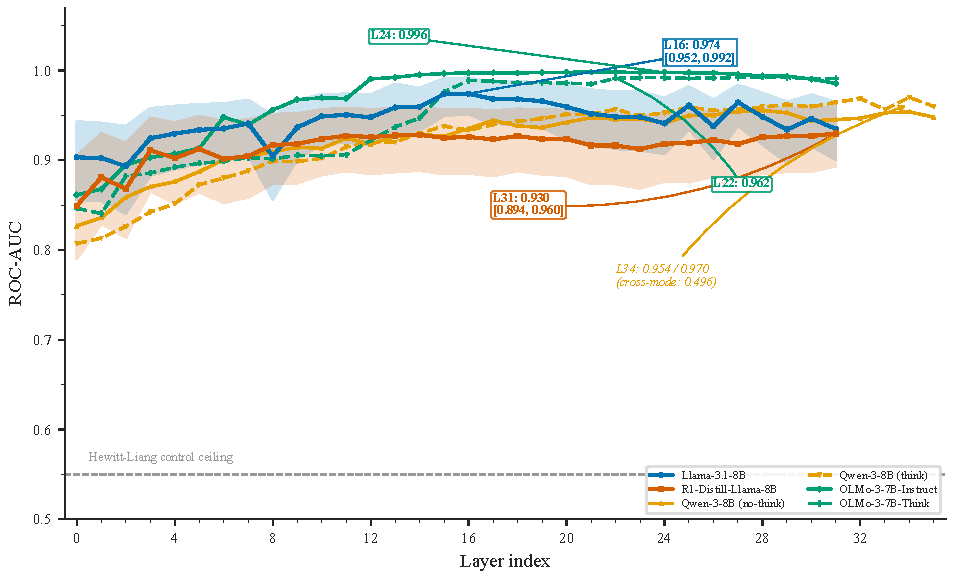
\includegraphics[width=0.85\linewidth]{../figures/fig1_probe_auc_curves.pdf}
\vspace{-4pt}
\caption{Layer-wise probe ROC-AUC (conflict vs.\ no-conflict, three
  vulnerable categories).  Llama peaks at 0.974 [0.952, 0.992] (L16);
  R1-Distill at 0.930 [0.894, 0.960] (L31).
  Qwen~3-8B peaks at 0.954 (no-think) and 0.970 (think) at L34, but
  cross-mode transfer is at chance (0.496).
  Gray dashed: Hewitt--Liang control ceiling.}
\label{fig:probe_curves}
\end{figure}

Llama peaks at AUC\,=\,0.974 (95\% CI [0.952, 0.992]) at L16;
R1-Distill peaks lower at AUC\,=\,0.930 [0.894, 0.960] at L31 (CIs
overlap slightly but point estimates differ by 0.044).  The 15-layer shift
(L16\,$\to$\,L31 of 32) is architecturally suggestive: Llama resolves
conflict in the middle of the network, leaving later layers to map the
resolution to vocabulary tokens for an immediate answer; R1-Distill pushes
the conflict representation to the penultimate layer where its primary
downstream operation is to initialize the chain-of-thought rollout rather
than produce an answer directly \citep{zhang2025probing}.
Qwen~3-8B achieves high separability in both modes (no-think: 0.954; think: 0.970; both at L34), but cross-mode probe transfer is at chance (AUC\,=\,0.496, cosine $= -0.005$): probes trained in one mode do not generalize to the other.  Because the no-think template injects four tokens before \pzero{} (Section~\ref{sec:methods}), the two modes' \pzero{} positions differ in both absolute index and local context, guaranteeing a geometric subspace rotation via RoPE and attention to the injected tokens.  The non-transferability is therefore an expected consequence of the template difference.  Each mode independently achieves high within-mode separability (${\sim}$0.97), yet the model must use the CoT to navigate from the think-mode subspace to the correct answer.

\paragraph{Selectivity and text-only baseline.}  Hewitt--Liang control probes achieve
AUC\,$\leq$\,0.66 at all layers, indicating that the true probes
decode representational content, not probe capacity.  Selectivity
exceeds 34 percentage points at peak layers for both models.\footnote{We
  train probes in two settings: 5-fold CV on all 350 items (7 categories,
  peak L14, AUC\,=\,0.999), used for cross-prediction and steering; and
  bootstrap CI analysis on 160 vulnerable-category items (3 categories,
  peak L16, AUC\,=\,0.974 [0.952, 0.992]).}
Three text-only baselines cluster in a narrow band: a
length-only probe (word count, 5-fold CV) achieves AUC\,=\,0.863,
a TF-IDF unigram+bigram logistic regression achieves 0.820, and a
global sentence-transformer baseline achieves 0.840, all substantially
below the activation probe (0.999).  All three per-category syllogism
results collapse to below chance ($\leq$0.086), because
conflict and control syllogisms are surface-matched in length ($d\!=\!+0.02$)
and vocabulary; the activation probe remains at 0.999.  The
narrow 0.82--0.86 text-baseline band shows the \textasciitilde16pp
gap to the activation probe reflects information absent from input
text, regardless of text-encoding method.

\paragraph{Probe summary.}
Table~\ref{tab:probe_summary} summarizes the key probing metrics.

\begin{table}[t]
\centering
\caption{Probing summary at peak layer for the three
  vulnerable categories.  95\% CIs: bootstrap (1000 resamples) for
  Llama/R1/OLMo-7B rows; CV-fold $\pm 1.96\sigma$ for OLMo-32B rows
  (${}^\dagger$; per-sample predictions not cached for bootstrap).
  Qwen CIs omitted (only layer-level aggregates stored).
  Layer-selection uncertainty is not propagated in any row.
  Selectivity = true AUC $-$ control AUC.  Cross-mode column:
  AUC when a probe trained on one Qwen mode is tested on the other.
  Text baselines: three methods on input text only (no activations)---see range in last row.}
\label{tab:probe_summary}
\vspace{4pt}
\small
\begin{tabular}{lcccccc}
\toprule
\textbf{Model} & \textbf{Peak L} & \textbf{Peak AUC} & \textbf{95\% CI} & \textbf{Ctrl AUC} & \textbf{Select.} & \textbf{Cross} \\
\midrule
Llama-3.1-8B-Instruct & L16 & 0.974 & [0.952, 0.992] & 0.63 & 0.343 & --- \\
R1-Distill-Llama-8B   & L31 & 0.930 & [0.894, 0.960] & 0.55 & 0.377 & --- \\
Qwen~3-8B (no think)  & L34 & 0.954 & ---             & ---  & --- & 0.496 \\
Qwen~3-8B (think)     & L34 & 0.970 & ---             & ---  & --- & 0.496 \\
\midrule
OLMo-3-7B-Instruct    & L24 & 0.996 & [0.988, 1.000]  & ---  & --- & --- \\
OLMo-3-7B-Think       & L22 & 0.962 & [0.934, 0.982]  & ---  & --- & --- \\
\midrule
OLMo-3.1-32B-Instruct & L20 & 0.9999 & $[0.9997, 1.000]^\dagger$ & --- & --- & --- \\
OLMo-3.1-32B-Think    & L20 & 0.9978 & $[0.9960, 0.9996]^\dagger$ & --- & --- & --- \\
\midrule
\emph{Text baselines}  & --- & 0.820--0.863 & ---         & ---  & --- & --- \\
\bottomrule
\end{tabular}
\end{table}

\paragraph{Cross-prediction and immune-category specificity.}
Training on \emph{vulnerable} categories and testing on \emph{immune} categories yields near-chance transfer.  ROC-AUC is ill-defined here because immune items are processed equivalently regardless of the conflict label, collapsing processing-mode variance to near zero; logit histograms confirm that immune items compress into a tight cluster (spread $0.03\times$ that of vulnerable categories).  Base rate and conjunction probes transfer near-perfectly to each other (AUC\,$>$\,0.99), while transfer to syllogism is weaker (0.59--0.63).

\paragraph{Cross-model probe transfer.}
A Llama-trained probe achieves AUC\,=\,0.920 on R1-Distill (layer~23, the peak transfer layer from a full 32-layer sweep); the reverse achieves 0.954 at layer~15 (also the peak transfer layer from a full sweep).  The processing-mode direction is substantially shared across models differing only in reasoning training, contrasting with \citet{huang2026cogbias}'s near-orthogonal finding across architectures.

\paragraph{Lure susceptibility scores.}
Llama's mean \pzero{} logit score for the S1-lure answer is $+0.422$
(the lure answer is favored in the pre-generation representation),
while R1-Distill's mean is $-0.326$ (the correct answer is favored).
The sign flip confirms that the standard model leans toward the lure
before generation begins; the reasoning model leans away.

% ---------------------------------------------------------------
\subsection{Causal Evidence: Probe-Direction Steering}
\label{sec:steering}

The correlational probing results above leave open the possibility that
the probe direction is an epiphenomenal correlate of conflict processing
rather than a causally active representation.  We test this directly by
steering Llama-3.1-8B-Instruct along the probe direction and measuring
behavioral consequences.

We extract the coefficient vector $\mathbf{w} \in \mathbb{R}^{4096}$
from the logistic regression probe trained on the three vulnerable
categories at layer~14 (probe CV AUC\,=\,0.960) and normalize it to
$\hat{\mathbf{w}} = \mathbf{w} / \|\mathbf{w}\|$.  At inference time, we
add $\alpha \cdot \hat{\mathbf{w}}$ to the residual stream at L14,
sweeping $\alpha \in \{-5, -3, -1, 0, +1, +3, +5\}$ across all 80
vulnerable-category conflict items.  Positive $\alpha$ steers toward the
\stwo{} (correct) pole; negative $\alpha$ steers toward \sone{} (lure).
The probe is trained via 5-fold CV on the same 160-item set; the steering
evaluation is a held-in behavioral test, not a held-out split.  The causal
claim rests on the direction-specificity controls below, not on held-out
generalization.

Figure~\ref{fig:steering} shows a monotonic dose-response: at $\alpha = -5$ (toward \sone{}), lure rate rises to 68.8\%; at $\alpha = +5$ (toward \stwo{}), it drops to 31.2\%---a 37.5pp causal swing, comparable to \citet{huang2026cogbias}'s 26--32\% reduction.  The entire lure reduction converts to correct answers (zero increase in ``other'' responses), ruling out distributional disruption.  Random-direction controls (50 unit vectors per $\alpha$) show no systematic effect (mean lure 52--57\%, $\sigma \leq 8.7$pp per endpoint); the probe's 37.5pp swing exceeds $3\sigma$ of the random-swing distribution ($\sigma_{\text{swing}} = \sigma\sqrt{2} \approx 12.3$pp).

\paragraph{Two specificity controls.}
(i)~Probe steering on matched \emph{non-conflict} items produces zero lure responses at any $\alpha$, with only minor coherence loss at $|\alpha|\!=\!5$ (Appendix~\ref{app:steering_specificity}): the direction is specific to the conflict subspace.  (ii)~The CogBias-style mean-difference vector (cosine $= 0.314$ with the probe) is a stronger one-sided debiasing intervention (lure 52.5\%$\to$11.25\% at $\alpha\!=\!+5$) but is \emph{unidirectional}---negative $\alpha$ has no effect (stays 53.75\%).  The probe direction is weaker for debiasing but \emph{bidirectional} ($+$16.25pp worse at $\alpha\!=\!-5$), making it better evidence of a causal boundary.

\paragraph{R1-Distill steering contrast: layer sweep.}
We sweep four layers in R1-Distill (L14, L25, L28, L31) under continuous
steering across the full 2048-token generation, directly addressing the
objection that steering at L14 (Llama's peak) may miss a deeper writable
locus in R1 (whose probe peaks at L31).  Table~\ref{tab:r1_layer_sweep_anon}
shows the result: \emph{no layer produces a coherent dose-response.}
Lure rate fluctuates between 6--14\% with no monotonic trend at any
layer.  At L31 (R1's probe peak, AUC\,=\,0.930), lure is 10.0\% at
$\alpha\!=\!-5$ and 11.25\% at $\alpha\!=\!+5$ (endpoint-to-endpoint
swing of 1.25pp; full sweep range 5.0pp), compared to Llama's 37.5pp
endpoint swing (Figure~\ref{fig:steering}).  The model
remains fluent at all layers and all $\alpha$ (correct rate $\geq 86\%$,
``other'' rate $\leq 14\%$, dropping to exactly 0\% at L31); the other-response rate provides an upper bound on incoherent or bypassed outputs.
The direction that is causally active in Llama is not stably controllable
in R1-Distill at \emph{any} layer: \emph{readable but not writable.}

\begin{table}[t]
\centering
\caption{R1-Distill layer-sweep steering (continuous, 80 vulnerable
  conflict items).  Lure rate (\%) at each $\alpha$; no layer
  shows a monotonic dose-response (full-sweep ranges: L14\,=\,8.8pp,
  L25\,=\,7.6pp, L28\,=\,5.0pp, L31\,=\,5.0pp; endpoint swing at
  L31: $10.0\%\to11.25\%=1.25$pp).  Compare Llama L14: 68.8\%$\to$31.2\%
  (37.5pp endpoint swing).}
\label{tab:r1_layer_sweep_anon}
\vspace{4pt}
\small
\begin{tabular}{l rrrrrrr}
\toprule
\textbf{Layer} & $-5$ & $-3$ & $-1$ & $0$ & $+1$ & $+3$ & $+5$ \\
\midrule
L14 & 6.2 & 10.0 & 7.5 & 6.2 & 5.0 & 7.5 & 13.8 \\
L25 & 6.2 & 6.2 & 8.8 & 11.2 & 10.0 & 13.8 & 8.8 \\
L28 & 8.8 & 6.2 & 10.0 & 11.2 & 7.5 & 11.2 & 10.0 \\
L31 & 10.0 & 6.2 & 10.0 & 11.2 & 10.0 & 8.8 & 11.2 \\
\bottomrule
\end{tabular}
\end{table}

\begin{figure}[t]
\centering
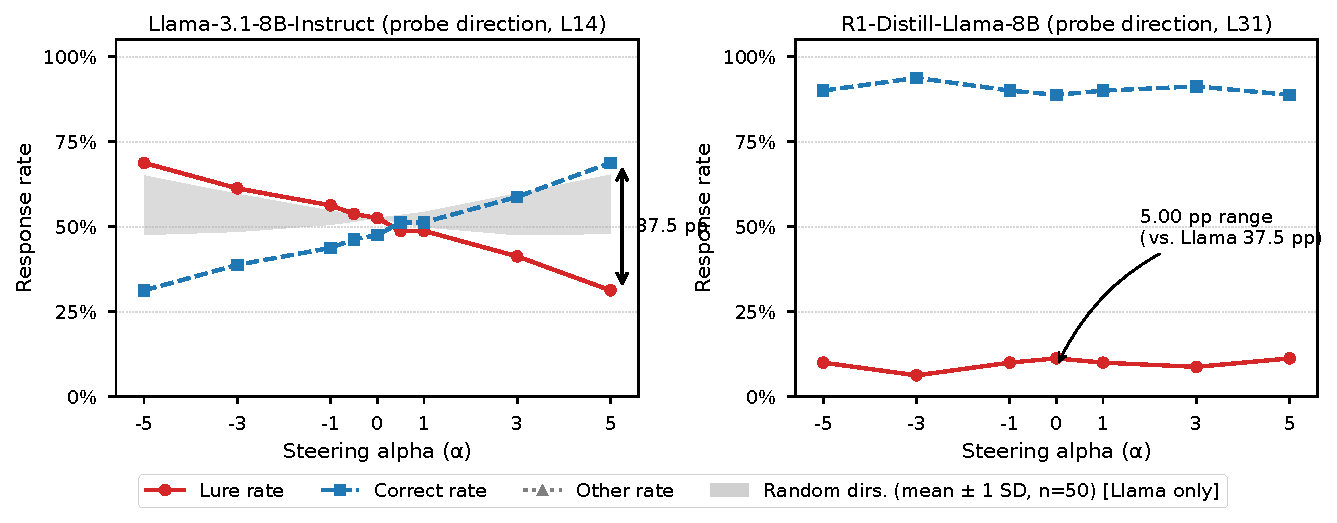
\includegraphics[width=\linewidth]{../figures/fig_steering_llama_r1_comparison.pdf}
\vspace{-4pt}
\caption{Probe-direction steering (80 vulnerable-category conflict items).
  \emph{Left}: Llama-3.1-8B-Instruct (L14) shows a 37.5pp dose-response
  ($\alpha\!=\!-5$: 68.8\% lure; $\alpha\!=\!+5$: 31.2\%),  with 100\% of
  lure reduction converting to correct answers (other rate stays 0);
  50 random directions (gray band, $n\!=\!50$) show no systematic effect.
  \emph{Right}: R1-Distill-Llama-8B (L31, its probe-peak layer) shows
  no coherent dose-response (5.0pp range, compared to Llama's 37.5pp):
  the probe direction is readable but not writable.}
\label{fig:steering}
\end{figure}

% ---------------------------------------------------------------
\subsection{Within-CoT Probing}
\label{sec:within_cot}

\begin{figure}[t]
\centering
\vspace{-6pt}
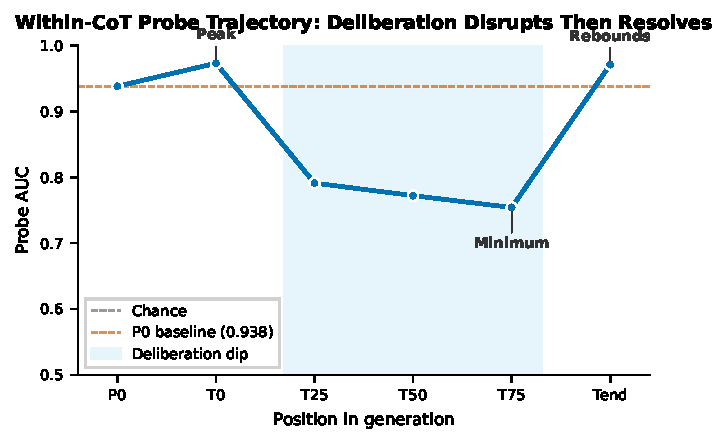
\includegraphics[width=0.78\linewidth]{../figures/fig_within_cot_trajectory.pdf}
\vspace{-6pt}
\caption{Within-CoT probe AUC for Qwen~3-8B (think mode) at L34.
  Three phases: \emph{crystallization} (P0$\to$T0, +3.5pp),
  \emph{exploration} (T0$\to$T75, $-$22pp dip),
  \emph{resolution} (T75$\to$Tend, full rebound to 0.971).
  P2 (control) = 0.500.}
\label{fig:within_cot}
\end{figure}

We probe residual stream activations at seven canonical positions
for Qwen~3-8B (think mode) at L34 (Figure~\ref{fig:within_cot}).
Probe AUC follows a non-monotonic U-shape: P0 (0.938) $\to$ T0 (0.973)
$\to$ T75 (0.754) $\to$ Tend (0.971); P2 = 0.500 (chance).
Three phases: \emph{crystallization} (thinking onset sharpens by +3.5pp
before substantive reasoning); \emph{exploration} (AUC drops ${\sim}22$pp
as mid-trace representations explore alternative framings); \emph{resolution}
(rebound to 0.971 before answer generation).
This rules out flat ``performative reasoning'' (22pp dip) and monotonic
sharpening (T0$>$T50 inversion) \citep{boppana2026reasoning,jiang2025aha}.
Full trajectories in Appendix~\ref{app:within_cot}.

% ---------------------------------------------------------------
\subsection{Scale Analysis: 7B vs.\ 32B}
\label{sec:scale}

OLMo-3.1-32B-Instruct shows \emph{more} vulnerability than 7B
(19.6\% vs.\ 14.9\%), mirroring inverse-scaling phenomena
\citep{mckenzie2023inverse, perez2023discovering}; Think collapses
lure to 0.4\%.  The behavioral gap \emph{widens} with scale (19.2pp
at 32B vs.\ 14.0pp at 7B) while the probe-AUC gap \emph{shrinks}
(0.0021 vs.\ 0.0055), further evidence for readable but not writable.
Full breakdowns in Appendix~\ref{app:scale}.

% ---------------------------------------------------------------
\subsection{SAE Features and Attention Entropy}
\label{sec:results_sae_attention}

SAE analysis of Llama's L19 residual stream identified 41 features with
significant conflict/control differential activation (BH-FDR $q < 0.05$),
all surviving Ma et al.\ falsification \citep{ma2026falsification}: 19
fire exclusively on conflict items, 6 on controls, with interpretable
token-level triggers.  R1-Distill has nearly twice as many
\stwo{}-specialized attention heads (57 vs.\ 30 of 1024; BH-FDR
$q < 0.05$, $|r_{rb}| \geq 0.3$).  Details in
Appendix~\ref{app:sae_attention}.

% ============================================================
% 6. Discussion (~1.5 pages)
% ============================================================

\section{Discussion}
\label{sec:discussion}

\paragraph{Conflict detection without resolution.}
The standard model \emph{detects} conflict (AUC\,=\,0.974) yet fails
to resolve it (27.3\% lure rate), paralleling De~Neys'
\citep{deneys2012bias} finding that human conflict monitoring occurs
even when the heuristic prevails.
The reasoning model shows \emph{less} distinct encoding (AUC\,=\,0.930)
yet much better resolution (2.4\%), replicated in OLMo
(AUC 0.996 $\to$ 0.962; lure 14.9\% $\to$ 0.9\%), consistent with
reasoning distillation automating Type~2 processing
\citep{evans2019reflections, venhoff2025base}.

\paragraph{Readable but not writable.}
In Llama, the probe direction is readable (AUC\,=\,0.974) and writable
(37.5pp causal swing); in R1-Distill, it is readable (AUC\,=\,0.930)
but not detectably writable at any of four layers under continuous
2048-token intervention.  The within-CoT trajectory
(Section~\ref{sec:within_cot}) offers a mechanistic explanation: the
conflict representation rotates during deliberation (AUC drops to 0.754
at T75), so a static \pzero{} steering vector becomes misaligned with
the evolving CoT subspace.  The bias direction in R1-Distill is in
this sense \emph{vestigial}: decoupled from the behavioral output pathway.
Limitations include reliance on linear probes (which may miss nonlinear
structure), a single steering direction per model, and restriction to
$\leq$32B English-language models.  Five controls
\citep{meloux2025dead, sanitychecks2026} guard against artifacts
(Appendix~\ref{app:robustness}).

% ============================================================
% References
% ============================================================
\bibliographystyle{plainnat}
\bibliography{references}

% ============================================================
% Appendix (does not count toward page limit)
% ============================================================

\appendix

\section{Within-CoT Probing Details}
\label{app:within_cot}

This appendix details the within-chain-of-thought probing protocol
for Qwen~3-8B (think mode).  For each model--item pair, we extract
residual stream activations at five canonical positions within the
\texttt{<think>...\allowbreak</think>} trace: T0 (first token), T25,
T50, T75, and Tend (final token before \texttt{</think>}).  We train
independent $\ell_2$-regularized logistic regression probes (5-fold
stratified CV) at each (layer, position) combination on the conflict
vs.\ no-conflict classification ($n = 160$).

\begin{table}[ht]
\centering
\caption{Within-CoT probe AUC trajectory for Qwen~3-8B (think mode)
  at L34, 7 positions.}
\label{tab:within_cot_qwen}
\vspace{4pt}
\small
\begin{tabular}{lcc}
\toprule
\textbf{Position} & \textbf{Description} & \textbf{Probe AUC} \\
\midrule
P0   & Pre-generation          & 0.938 \\
T0   & Thinking onset          & \textbf{0.973} \\
T25  & 25\% of trace           & 0.791 \\
T50  & Midpoint                & 0.772 \\
T75  & 75\% of trace           & 0.754 \\
Tend & Final thinking token    & 0.971 \\
P2   & Control (chance)        & 0.500 \\
\bottomrule
\end{tabular}
\end{table}

The U-shaped trajectory (T0 peak, T25--T75 dip, Tend rebound) rules
out both performative reasoning (flat AUC) and monotonic sharpening.
The orthogonal \pzero{} directions between Qwen's think/no-think modes
(cross-mode AUC\,=\,0.496) combined with genuine representational work
during the trace show that training and inference-time thinking are
mechanistically distinct: training reorganizes the encoding, while
thinking operates within an orthogonal encoding to resolve conflicts
during generation.

\section{Scale Analysis: Full Results}
\label{app:scale}

OLMo-3.1-32B-Instruct/Think (64 layers, 5120 hidden dims) were evaluated
on the full 470-item benchmark.  Lure rate rises from 14.9\% (7B) to
19.6\% (32B Instruct), with base rate neglect doubling (46\%$\to$74.3\%).
Reasoning training at 32B drops lure to 0.4\%.  Probes achieve
AUC\,=\,0.9999 (Instruct L20) and 0.9978 (Think L20): the behavioral gap
widens (19.2pp at 32B vs.\ 14.0pp at 7B) while the representational gap
shrinks (0.0021 vs.\ 0.0055).

\section{SAE Features and Attention Entropy}
\label{app:sae_attention}
Full SAE feature analysis (41 significant features, Ma et al.\
falsification details) and per-head attention entropy results.

\section{Multi-Seed Robustness}
\label{app:robustness}
Multi-seed evaluation with sampled decoding (temperature 0.7) shows
that Llama's overall lure rate remains stable (27.5\% $\pm$ 1.3pp across
3 seeds), but category profiles shift.  Probe results at \pzero{} are
unaffected by generation strategy, as they measure the pre-decision
representation.

\subsection{Exact Generation Parameters}

Table~\ref{tab:gen_kwargs} reports the exact generation keyword arguments
used for each model family.

\begin{table}[ht]
\centering
\caption{Generation keyword arguments for all models.  ``Greedy'' denotes
  the main-text configuration; ``Sampled'' denotes the robustness
  configuration used in this appendix.}
\label{tab:gen_kwargs}
\vspace{4pt}
\small
\begin{tabular}{lll}
\toprule
\textbf{Parameter} & \textbf{Greedy (main text)} & \textbf{Sampled (this appendix)} \\
\midrule
\texttt{do\_sample}       & \texttt{False} & \texttt{True} \\
\texttt{temperature}      & 1.0            & 0.7 \\
\texttt{top\_p}           & ---            & 0.95 \\
\texttt{max\_new\_tokens} & 128 (standard) / 2048 (reasoning) & same \\
System prompt             & none           & none \\
\bottomrule
\end{tabular}
\end{table}

\paragraph{Vendor-recommended settings.}
Our greedy configuration departs from several vendor recommendations:
DeepSeek recommends \texttt{temperature=0.5--0.7} for R1 models;
Qwen recommends \texttt{temperature=0.6} with \texttt{top\_p=0.95}
for Qwen~3.  We use deterministic greedy decoding throughout the main
text to (a)~ensure exact reproducibility without seed dependence,
(b)~isolate representational differences from generation-strategy
effects, and (c)~simplify the probing analysis, since \pzero{}
activations are deterministic given the prompt regardless of downstream
sampling.  This appendix demonstrates that the qualitative findings---
in particular the S1/S2 lure-rate gap and the stability of probe AUC
at \pzero{}---are preserved under vendor-recommended sampled decoding
(\texttt{temperature=0.7}).

\paragraph{Robustness argument.}
The key robustness claim is twofold: (1)~probe results at \pzero{}
are \emph{invariant} to generation strategy because \pzero{} activations
depend only on the prompt, not on downstream sampling; and
(2)~behavioral lure-rate gaps between S1 and S2 models are qualitatively
preserved under sampled decoding, though the magnitudes shift for
reasoning models whose chain-of-thought is sensitive to stochastic
token selection.

% =========================================================================
\section{Token-Length Confound Analysis}
\label{app:length_anon}

Near-perfect probe AUC (e.g., OLMo-32B at 0.9999) can in principle
arise from trivial confounds like systematic prompt-length differences
between conflict and control items.  Table~\ref{tab:length_anon}
reports subword token counts per category using the Llama-3.1-8B
tokenizer.

\begin{table}[ht]
\centering
\caption{Prompt subword length (Llama-3.1-8B tokenizer) for
  conflict vs.\ control items by category.  ``$d$'' is Cohen's~$d$;
  positive values indicate conflict items are longer.}
\label{tab:length_anon}
\vspace{4pt}
\small
\begin{tabular}{lrrrr}
\toprule
\textbf{Category} & \textbf{Conflict} & \textbf{Control} & \textbf{Cohen's $d$} & \textbf{$p$} \\
\midrule
Base rate      & 98.0  & 66.7  & $+3.69$  & $<10^{-4}$ \\
Conjunction    & 87.7  & 63.4  & $+6.36$  & $<10^{-4}$ \\
Syllogism      & 93.3  & 93.2  & $+0.02$  & 0.953 \\
CRT            & 47.0  & 51.8  & $-0.44$  & 0.097 \\
Arithmetic     & 70.9  & 51.0  & $+6.21$  & $<10^{-4}$ \\
Framing        & 97.2  & 106.2 & $-4.86$  & $<10^{-4}$ \\
Anchoring      & 60.4  & 45.5  & $+4.62$  & $<10^{-4}$ \\
\midrule
\textbf{Overall} & \textbf{81.1} & \textbf{68.4} & $+0.45$ & $<10^{-4}$ \\
\bottomrule
\end{tabular}
\end{table}

\paragraph{Why length is not the primary signal.}
Length differences are substantial on base rate and conjunction but
balanced on syllogism and reversed on framing.  Three observations
rule out length as the dominant confound.  First, a probe trained on
syllogism alone (where length is balanced, $d\!=\!+0.02$) achieves
within-category AUC\,=\,0.936 and transfers to base rate (0.950) and
conjunction (0.990)---the shared direction cannot be length.  Second,
length direction is inconsistent across categories, so a pure-length
probe would produce anti-correlated cross-category predictions rather
than the immune-cluster compression we observe.  Third, the text
baseline, which has direct access to length as a feature, caps at
0.840; the 16\,pp gap to the activation probe (0.999) cannot come from
length.  For OLMo-32B specifically, probe AUC\,=\,0.9999 on the
three vulnerable categories (including length-balanced syllogism)
implies the probe separates syllogism conflict vs.\ control despite
near-identical prompt lengths (93.3 vs.\ 93.2 tokens).

% =========================================================================
\section{Full Behavioral Breakdown (All Models, All Categories)}
\label{app:full_behavior_anon}

Table~\ref{tab:behavioral-full} provides the complete behavioral
breakdown for all eight evaluated models and eleven categories, with
conflict accuracy (Acc), lure rate (Lure), other-response rate (Other),
matched-control accuracy (Ctrl), and accuracy gap ($=$ Ctrl\,$-$\,Acc).
Wilson 95\% CIs in brackets.  The final column reports McNemar mid-$p$
on conflict vs.\ matched-control accuracy, exploiting the paired
structure of the benchmark.  Dashes indicate categories not evaluated
on a particular model.

% Full behavioral results table -- correct/lure/other rates
% Generated: 2026-04-15T05:22:48.779708+00:00
% Script: scripts/compute_full_behavior_table.py

\begin{table*}[t]
\centering
\caption{Complete behavioral results across models and categories. Conflict accuracy (Acc), lure rate (Lure), and other-response rate (Other) on conflict items; control accuracy (Ctrl); and accuracy gap (Gap = Ctrl $-$ Acc). Wilson 95\% CIs in brackets. McNemar mid-$p$ tests conflict vs.\ matched control accuracy.}
\label{tab:behavioral-full}
\scriptsize
\setlength{\tabcolsep}{3pt}
\begin{tabular}{l l r r r r r r r r r r r r}
\toprule
Model & Metric & CRT & Base Rate & Conjunction & Syllogism & Arithmetic & Framing & Anchoring & Sunk Cost & Availability & Certainty Eff. & Loss Aversion & Overall \\
\midrule
Llama-3.1-8B & Acc & 93.3\%\,{\tiny [79,98]} & 16.0\%\,{\tiny [6,35]} & 45.0\%\,{\tiny [26,66]} & 48.0\%\,{\tiny [30,67]} & 100.0\%\,{\tiny [87,100]} & 100.0\%\,{\tiny [84,100]} & 50.0\%\,{\tiny [30,70]} & --- & --- & --- & --- & 65.5\%\,{\tiny [58,72]} \\
 & Lure & 0.0\%\,{\tiny [0,11]} & \textbf{84.0\%\,{\tiny [65,94]}} & \textbf{55.0\%\,{\tiny [34,74]}} & \textbf{52.0\%\,{\tiny [33,70]}} & 0.0\%\,{\tiny [0,13]} & 0.0\%\,{\tiny [0,16]} & 0.0\%\,{\tiny [0,16]} & --- & --- & --- & --- & \textbf{27.3\%\,{\tiny [21,35]}} \\
 & Other & 6.7\% & 0.0\% & 0.0\% & 0.0\% & 0.0\% & 0.0\% & 50.0\% & --- & --- & --- & --- & 7.3\% \\
 & Ctrl & 90.0\%\,{\tiny [74,97]} & 100.0\%\,{\tiny [87,100]} & 100.0\%\,{\tiny [84,100]} & 52.0\%\,{\tiny [33,70]} & 100.0\%\,{\tiny [87,100]} & 100.0\%\,{\tiny [84,100]} & 80.0\%\,{\tiny [58,92]} & --- & --- & --- & --- & 88.5\%\,{\tiny [83,93]} \\
 & Gap & -3.3pp & +84.0pp & +55.0pp & +4.0pp & +0.0pp & +0.0pp & +30.0pp & --- & --- & --- & --- & +23.0pp ($p < .001$) \\
\midrule
R1-Distill-8B & Acc & 83.3\%\,{\tiny [66,93]} & 16.0\%\,{\tiny [6,35]} & 100.0\%\,{\tiny [84,100]} & 100.0\%\,{\tiny [87,100]} & 96.0\%\,{\tiny [80,99]} & 100.0\%\,{\tiny [84,100]} & 65.0\%\,{\tiny [43,82]} & --- & --- & --- & --- & 79.4\%\,{\tiny [73,85]} \\
 & Lure & 3.3\%\,{\tiny [1,17]} & 4.0\%\,{\tiny [1,20]} & 0.0\%\,{\tiny [0,16]} & 0.0\%\,{\tiny [0,13]} & 0.0\%\,{\tiny [0,13]} & 0.0\%\,{\tiny [0,16]} & 10.0\%\,{\tiny [3,30]} & --- & --- & --- & --- & 2.4\%\,{\tiny [1,6]} \\
 & Other & 13.3\% & 80.0\% & 0.0\% & 0.0\% & 4.0\% & 0.0\% & 25.0\% & --- & --- & --- & --- & 18.2\% \\
 & Ctrl & 100.0\%\,{\tiny [89,100]} & 16.0\%\,{\tiny [6,35]} & 100.0\%\,{\tiny [84,100]} & 96.0\%\,{\tiny [80,99]} & 100.0\%\,{\tiny [87,100]} & 100.0\%\,{\tiny [84,100]} & 65.0\%\,{\tiny [43,82]} & --- & --- & --- & --- & 82.4\%\,{\tiny [76,87]} \\
 & Gap & +16.7pp & +0.0pp & +0.0pp & -4.0pp & +4.0pp & +0.0pp & +0.0pp & --- & --- & --- & --- & +3.0pp ($p = 0.15$) \\
\midrule
Qwen3-8B {\small(no think)} & Acc & 73.3\%\,{\tiny [56,86]} & 44.0\%\,{\tiny [27,63]} & 5.0\%\,{\tiny [1,24]} & 48.0\%\,{\tiny [30,67]} & 100.0\%\,{\tiny [87,100]} & 100.0\%\,{\tiny [84,100]} & 80.0\%\,{\tiny [58,92]} & --- & --- & --- & --- & 64.8\%\,{\tiny [57,72]} \\
 & Lure & 0.0\%\,{\tiny [0,11]} & \textbf{56.0\%\,{\tiny [37,73]}} & \textbf{95.0\%\,{\tiny [76,99]}} & 0.0\%\,{\tiny [0,13]} & 0.0\%\,{\tiny [0,13]} & 0.0\%\,{\tiny [0,16]} & 10.0\%\,{\tiny [3,30]} & --- & --- & --- & --- & \textbf{21.2\%\,{\tiny [16,28]}} \\
 & Other & 26.7\% & 0.0\% & 0.0\% & 52.0\% & 0.0\% & 0.0\% & 10.0\% & --- & --- & --- & --- & 13.9\% \\
 & Ctrl & 100.0\%\,{\tiny [89,100]} & 100.0\%\,{\tiny [87,100]} & 100.0\%\,{\tiny [84,100]} & 52.0\%\,{\tiny [33,70]} & 100.0\%\,{\tiny [87,100]} & 100.0\%\,{\tiny [84,100]} & 65.0\%\,{\tiny [43,82]} & --- & --- & --- & --- & 88.5\%\,{\tiny [83,93]} \\
 & Gap & +26.7pp & +56.0pp & +95.0pp & +4.0pp & +0.0pp & +0.0pp & -15.0pp & --- & --- & --- & --- & +23.6pp ($p < .001$) \\
\midrule
Qwen3-8B {\small(think)} & Acc & 76.7\%\,{\tiny [59,88]} & 96.0\%\,{\tiny [80,99]} & 45.0\%\,{\tiny [26,66]} & 100.0\%\,{\tiny [87,100]} & 96.0\%\,{\tiny [80,99]} & 100.0\%\,{\tiny [84,100]} & 75.0\%\,{\tiny [53,89]} & --- & --- & --- & --- & 84.8\%\,{\tiny [79,90]} \\
 & Lure & 0.0\%\,{\tiny [0,11]} & 4.0\%\,{\tiny [1,20]} & \textbf{55.0\%\,{\tiny [34,74]}} & 0.0\%\,{\tiny [0,13]} & 0.0\%\,{\tiny [0,13]} & 0.0\%\,{\tiny [0,16]} & 0.0\%\,{\tiny [0,16]} & --- & --- & --- & --- & 7.3\%\,{\tiny [4,12]} \\
 & Other & 23.3\% & 0.0\% & 0.0\% & 0.0\% & 4.0\% & 0.0\% & 25.0\% & --- & --- & --- & --- & 7.9\% \\
 & Ctrl & 93.3\%\,{\tiny [79,98]} & 100.0\%\,{\tiny [87,100]} & 100.0\%\,{\tiny [84,100]} & 100.0\%\,{\tiny [87,100]} & 100.0\%\,{\tiny [87,100]} & 100.0\%\,{\tiny [84,100]} & 90.0\%\,{\tiny [70,97]} & --- & --- & --- & --- & 97.6\%\,{\tiny [94,99]} \\
 & Gap & +16.7pp & +4.0pp & +55.0pp & +0.0pp & +4.0pp & +0.0pp & +15.0pp & --- & --- & --- & --- & +12.7pp ($p < .001$) \\
\midrule
OLMo-3-7B-Instruct & Acc & 73.3\%\,{\tiny [56,86]} & 54.3\%\,{\tiny [38,70]} & 50.0\%\,{\tiny [30,70]} & 100.0\%\,{\tiny [87,100]} & 80.0\%\,{\tiny [61,91]} & 100.0\%\,{\tiny [84,100]} & 35.0\%\,{\tiny [18,57]} & 100.0\%\,{\tiny [80,100]} & 86.7\%\,{\tiny [62,96]} & 100.0\%\,{\tiny [80,100]} & 66.7\%\,{\tiny [42,85]} & 74.9\%\,{\tiny [69,80]} \\
 & Lure & 3.3\%\,{\tiny [1,17]} & \textbf{45.7\%\,{\tiny [30,62]}} & \textbf{50.0\%\,{\tiny [30,70]}} & 0.0\%\,{\tiny [0,13]} & 0.0\%\,{\tiny [0,13]} & 0.0\%\,{\tiny [0,16]} & 5.0\%\,{\tiny [1,24]} & 0.0\%\,{\tiny [0,20]} & \textbf{13.3\%\,{\tiny [4,38]}} & 0.0\%\,{\tiny [0,20]} & \textbf{33.3\%\,{\tiny [15,58]}} & \textbf{14.9\%\,{\tiny [11,20]}} \\
 & Other & 23.3\% & 0.0\% & 0.0\% & 0.0\% & 20.0\% & 0.0\% & 60.0\% & 0.0\% & 0.0\% & 0.0\% & 0.0\% & 10.2\% \\
 & Ctrl & 90.0\%\,{\tiny [74,97]} & 100.0\%\,{\tiny [90,100]} & 100.0\%\,{\tiny [84,100]} & 100.0\%\,{\tiny [87,100]} & 96.0\%\,{\tiny [80,99]} & 100.0\%\,{\tiny [84,100]} & 50.0\%\,{\tiny [30,70]} & 0.0\%\,{\tiny [0,20]} & 40.0\%\,{\tiny [20,64]} & 100.0\%\,{\tiny [80,100]} & 100.0\%\,{\tiny [80,100]} & 83.8\%\,{\tiny [79,88]} \\
 & Gap & +16.7pp & +45.7pp & +50.0pp & +0.0pp & +16.0pp & +0.0pp & +15.0pp & -100.0pp & -46.7pp & +0.0pp & +33.3pp & +8.9pp ($p = 0.014$) \\
\midrule
OLMo-3-7B-Think & Acc & 96.7\%\,{\tiny [83,99]} & 100.0\%\,{\tiny [90,100]} & 100.0\%\,{\tiny [84,100]} & 72.0\%\,{\tiny [52,86]} & 88.0\%\,{\tiny [70,96]} & 100.0\%\,{\tiny [84,100]} & 80.0\%\,{\tiny [58,92]} & 46.7\%\,{\tiny [25,70]} & 100.0\%\,{\tiny [80,100]} & 100.0\%\,{\tiny [80,100]} & 66.7\%\,{\tiny [42,85]} & 88.1\%\,{\tiny [83,92]} \\
 & Lure & 3.3\%\,{\tiny [1,17]} & 0.0\%\,{\tiny [0,10]} & 0.0\%\,{\tiny [0,16]} & 4.0\%\,{\tiny [1,20]} & 0.0\%\,{\tiny [0,13]} & 0.0\%\,{\tiny [0,16]} & 0.0\%\,{\tiny [0,16]} & 0.0\%\,{\tiny [0,20]} & 0.0\%\,{\tiny [0,20]} & 0.0\%\,{\tiny [0,20]} & 0.0\%\,{\tiny [0,20]} & 0.9\%\,{\tiny [0,3]} \\
 & Other & 0.0\% & 0.0\% & 0.0\% & 24.0\% & 12.0\% & 0.0\% & 20.0\% & 53.3\% & 0.0\% & 0.0\% & 33.3\% & 11.1\% \\
 & Ctrl & 93.3\%\,{\tiny [79,98]} & 100.0\%\,{\tiny [90,100]} & 100.0\%\,{\tiny [84,100]} & 68.0\%\,{\tiny [48,83]} & 100.0\%\,{\tiny [87,100]} & 100.0\%\,{\tiny [84,100]} & 70.0\%\,{\tiny [48,85]} & 0.0\%\,{\tiny [0,20]} & 100.0\%\,{\tiny [80,100]} & 100.0\%\,{\tiny [80,100]} & 13.3\%\,{\tiny [4,38]} & 81.3\%\,{\tiny [76,86]} \\
 & Gap & -3.3pp & +0.0pp & +0.0pp & -4.0pp & +12.0pp & +0.0pp & -10.0pp & -46.7pp & +0.0pp & +0.0pp & -53.3pp & -6.8pp ($p = 0.006$) \\
\midrule
OLMo-2-32B-Instruct & Acc & 86.7\%\,{\tiny [70,95]} & 25.7\%\,{\tiny [14,42]} & 50.0\%\,{\tiny [30,70]} & 96.0\%\,{\tiny [80,99]} & 96.0\%\,{\tiny [80,99]} & 70.0\%\,{\tiny [48,85]} & 70.0\%\,{\tiny [48,85]} & 100.0\%\,{\tiny [80,100]} & 100.0\%\,{\tiny [80,100]} & 100.0\%\,{\tiny [80,100]} & 100.0\%\,{\tiny [80,100]} & 77.0\%\,{\tiny [71,82]} \\
 & Lure & 6.7\%\,{\tiny [2,21]} & \textbf{74.3\%\,{\tiny [58,86]}} & \textbf{50.0\%\,{\tiny [30,70]}} & 0.0\%\,{\tiny [0,13]} & 0.0\%\,{\tiny [0,13]} & \textbf{30.0\%\,{\tiny [15,52]}} & 10.0\%\,{\tiny [3,30]} & 0.0\%\,{\tiny [0,20]} & 0.0\%\,{\tiny [0,20]} & 0.0\%\,{\tiny [0,20]} & 0.0\%\,{\tiny [0,20]} & \textbf{19.6\%\,{\tiny [15,25]}} \\
 & Other & 6.7\% & 0.0\% & 0.0\% & 4.0\% & 4.0\% & 0.0\% & 20.0\% & 0.0\% & 0.0\% & 0.0\% & 0.0\% & 3.4\% \\
 & Ctrl & 93.3\%\,{\tiny [79,98]} & 100.0\%\,{\tiny [90,100]} & 95.0\%\,{\tiny [76,99]} & 88.0\%\,{\tiny [70,96]} & 72.0\%\,{\tiny [52,86]} & 90.0\%\,{\tiny [70,97]} & 85.0\%\,{\tiny [64,95]} & 0.0\%\,{\tiny [0,20]} & 33.3\%\,{\tiny [15,58]} & 100.0\%\,{\tiny [80,100]} & 100.0\%\,{\tiny [80,100]} & 81.7\%\,{\tiny [76,86]} \\
 & Gap & +6.7pp & +74.3pp & +45.0pp & -8.0pp & -24.0pp & +20.0pp & +15.0pp & -100.0pp & -66.7pp & +0.0pp & +0.0pp & +4.7pp ($p = 0.25$) \\
\midrule
OLMo-2-32B-Think & Acc & 100.0\%\,{\tiny [89,100]} & 100.0\%\,{\tiny [90,100]} & 100.0\%\,{\tiny [84,100]} & 100.0\%\,{\tiny [87,100]} & 100.0\%\,{\tiny [87,100]} & 100.0\%\,{\tiny [84,100]} & 80.0\%\,{\tiny [58,92]} & 80.0\%\,{\tiny [55,93]} & 100.0\%\,{\tiny [80,100]} & 100.0\%\,{\tiny [80,100]} & 100.0\%\,{\tiny [80,100]} & 97.0\%\,{\tiny [94,99]} \\
 & Lure & 0.0\%\,{\tiny [0,11]} & 0.0\%\,{\tiny [0,10]} & 0.0\%\,{\tiny [0,16]} & 0.0\%\,{\tiny [0,13]} & 0.0\%\,{\tiny [0,13]} & 0.0\%\,{\tiny [0,16]} & 0.0\%\,{\tiny [0,16]} & 6.7\%\,{\tiny [1,30]} & 0.0\%\,{\tiny [0,20]} & 0.0\%\,{\tiny [0,20]} & 0.0\%\,{\tiny [0,20]} & 0.4\%\,{\tiny [0,2]} \\
 & Other & 0.0\% & 0.0\% & 0.0\% & 0.0\% & 0.0\% & 0.0\% & 20.0\% & 13.3\% & 0.0\% & 0.0\% & 0.0\% & 2.6\% \\
 & Ctrl & 100.0\%\,{\tiny [89,100]} & 100.0\%\,{\tiny [90,100]} & 100.0\%\,{\tiny [84,100]} & 100.0\%\,{\tiny [87,100]} & 100.0\%\,{\tiny [87,100]} & 100.0\%\,{\tiny [84,100]} & 85.0\%\,{\tiny [64,95]} & 0.0\%\,{\tiny [0,20]} & 100.0\%\,{\tiny [80,100]} & 100.0\%\,{\tiny [80,100]} & 80.0\%\,{\tiny [55,93]} & 91.1\%\,{\tiny [87,94]} \\
 & Gap & +0.0pp & +0.0pp & +0.0pp & +0.0pp & +0.0pp & +0.0pp & +5.0pp & -80.0pp & +0.0pp & +0.0pp & -20.0pp & -6.0pp ($p < .001$) \\
\bottomrule
\end{tabular}
\end{table*}


% =========================================================================
\section{Steering Specificity Controls}
\label{app:steering_specificity}

Table~\ref{tab:steering_specificity_anon} reports specificity controls
for Llama-3.1-8B-Instruct at L14.  Four sweeps: (1)~probe-direction on
conflict items (main result); (2)~probe-direction on matched non-conflict
control items (null-effect specificity); (3)~mean-difference direction
on conflict items (CogBias baseline); (4)~mean-difference on control.
cos(probe, mean-diff) $= 0.314$: the two directions differ substantially.

\begin{table}[ht]
\centering
\caption{Steering specificity controls on Llama-3.1-8B-Instruct, L14,
  continuous steering.  Conflict items carry an S1 lure answer;
  control items carry only the normative answer.}
\label{tab:steering_specificity_anon}
\vspace{4pt}
\small
\begin{tabular}{l l rrrrrrr}
\toprule
\textbf{Direction} & \textbf{Items} & $\alpha\!=\!-5$ & $-3$ & $-1$ & $0$ & $+1$ & $+3$ & $+5$ \\
\midrule
\multicolumn{9}{l}{\emph{Lure rate (\%)}} \\
Probe        & Conflict & 68.75 & 61.25 & 56.25 & 52.50 & 48.75 & 41.25 & 31.25 \\
Probe        & Control  & 0.00  & 0.00  & 0.00  & 0.00  & 0.00  & 0.00  & 0.00  \\
Mean-diff    & Conflict & 53.75 & 55.00 & 55.00 & 52.50 & 36.25 & 21.25 & 11.25 \\
Mean-diff    & Control  & 0.00  & 0.00  & 0.00  & 0.00  & 0.00  & 0.00  & 0.00  \\
\midrule
\multicolumn{9}{l}{\emph{Correct rate (\%)}} \\
Probe        & Conflict & 31.25 & 38.75 & 43.75 & 47.50 & 51.25 & 58.75 & 68.75 \\
Probe        & Control  & 78.75 & 87.50 & 98.75 & 100.00 & 100.00 & 100.00 & 100.00 \\
Mean-diff    & Conflict & 46.25 & 45.00 & 45.00 & 47.50 & 63.75 & 78.75 & 88.75 \\
Mean-diff    & Control  & 60.00 & 73.75 & 97.50 & 100.00 & 100.00 & 100.00 & 100.00 \\
\bottomrule
\end{tabular}
\end{table}

\paragraph{Three observations.}
(i) The probe direction produces \emph{zero} lure responses on control
items at any $\alpha$: the direction is specific to the S1/S2 conflict
subspace and does not generically perturb answers.  The small drop in
correctness at $\alpha\!=\!-5$ on control items (78.75\%) reflects
residual-stream coherence loss (the 21.25\% of items become ``other''
responses, not lures), the same pattern seen with random directions
in the main text.  (ii) The probe-weight direction is \emph{bidirectional}:
moving toward S1 (negative $\alpha$) increases lure by 16.25pp,
moving toward S2 (positive $\alpha$) decreases lure by 21.25pp.
Bidirectional dose-response is stronger evidence of causal sufficiency
than a unidirectional effect.  (iii) The mean-difference baseline is
\emph{unidirectional}: negative $\alpha$ has essentially no effect
(lure stays around 53--55\%), while positive $\alpha$ strongly
reduces lure (to 11.25\% at $\alpha\!=\!+5$).  Mean-difference
steering efficiently improves behavior but cannot test causal
sufficiency by worsening it---a key methodological motivation for
probe-weight steering.

% ============================================================
% NeurIPS Paper Checklist (required for submission)
% ============================================================
\section*{NeurIPS Paper Checklist}

\begin{enumerate}

\item {\bf Claims}
    \item[] Question: Do the main claims made in the abstract and introduction accurately reflect the paper's contributions and scope?
    \item[] Answer: \answerYes{}
    \item[] Justification: The abstract and introduction state three contributions—a 470-item benchmark, a multi-method mechanistic analysis (probes, SAEs, attention entropy, activation steering), and evidence for a graded deliberation-intensity dimension—all of which are supported by the experimental results presented in the paper.
\item {\bf Limitations}
    \item[] Question: Does the paper discuss the limitations of the work performed by the authors?
    \item[] Answer: \answerYes{}
    \item[] Justification: The Discussion section explicitly addresses limitations: experiments cover models up to 32B parameters (not frontier-scale), linear probes may miss nonlinear representational structure, and the benchmark is limited to English-language cognitive-bias tasks. We also discuss the inherent limitations of the dual-process operationalization.
\item {\bf Theory assumptions and proofs}
    \item[] Question: For each theoretical result, does the paper provide the full set of assumptions and a complete (and correct) proof?
    \item[] Answer: \answerNA{}
    \item[] Justification: This is an empirical study. The paper does not present theoretical results or proofs.
    \item {\bf Experimental result reproducibility}
    \item[] Question: Does the paper fully disclose all the information needed to reproduce the main experimental results of the paper to the extent that it affects the main claims and/or conclusions of the paper (regardless of whether the code and data are provided or not)?
    \item[] Answer: \answerYes{}
    \item[] Justification: We report all hyperparameters, cross-validation procedures (5-fold stratified CV), statistical methods (bootstrap CIs, BH-FDR correction), control tasks (Hewitt \& Liang random-label baselines, random-direction controls), model identifiers, and layer selections. The appendix contains full experimental details sufficient for independent replication.
\item {\bf Open access to data and code}
    \item[] Question: Does the paper provide open access to the data and code, with sufficient instructions to faithfully reproduce the main experimental results, as described in supplemental material?
    \item[] Answer: \answerYes{}
    \item[] Justification: Code and benchmark will be provided via anonymous link at review time. The 470-item benchmark (JSONL) and all analysis code will be released publicly upon acceptance.
\item {\bf Experimental setting/details}
    \item[] Question: Does the paper specify all the training and test details (e.g., data splits, hyperparameters, how they were chosen, type of optimizer) necessary to understand the results?
    \item[] Answer: \answerYes{}
    \item[] Justification: Section~4 and the appendix specify data splits (5-fold stratified CV by task category and label), probe hyperparameters (logistic regression with L2 regularization, selected via nested CV), SAE reconstruction fidelity thresholds, attention entropy normalization, and activation steering parameters. All models are identified by their HuggingFace IDs and accessed via publicly available weights.
\item {\bf Experiment statistical significance}
    \item[] Question: Does the paper report error bars suitably and correctly defined or other appropriate information about the statistical significance of the experiments?
    \item[] Answer: \answerYes{}
    \item[] Justification: All probe accuracy and AUC metrics are reported with bootstrap 95\% confidence intervals (1000 resamples). Multiple comparisons across layers and models are corrected with Benjamini-Hochberg FDR at $q=0.05$. Multi-seed robustness analyses report mean $\pm$ standard deviation across seeds. The source of variability (CV fold, bootstrap resample, or random seed) is stated for each metric.
\item {\bf Experiments compute resources}
    \item[] Question: For each experiment, does the paper provide sufficient information on the computer resources (type of compute workers, memory, time of execution) needed to reproduce the experiments?
    \item[] Answer: \answerYes{}
    \item[] Justification: The paper reports that all experiments were conducted on NVIDIA B200 GPUs via RunPod, with a total compute budget of approximately 100 GPU-hours. Per-workstream compute breakdowns are provided in the appendix.
\item {\bf Code of ethics}
    \item[] Question: Does the research conducted in the paper conform, in every respect, with the NeurIPS Code of Ethics \url{https://neurips.cc/public/EthicsGuidelines}?
    \item[] Answer: \answerYes{}
    \item[] Justification: The research uses only publicly available open-source models and does not involve human subjects, deception, or personally identifiable information. All work conforms to the NeurIPS Code of Ethics.
\item {\bf Broader impacts}
    \item[] Question: Does the paper discuss both potential positive societal impacts and negative societal impacts of the work performed?
    \item[] Answer: \answerYes{}
    \item[] Justification: The Discussion section addresses broader impacts: positively, our methods could inform runtime monitoring of LLM reasoning fidelity for AI safety; negatively, better understanding of internal deliberation could theoretically aid adversarial manipulation of model reasoning. We assess the risk as low given that the work is interpretability research on open-source models.
\item {\bf Safeguards}
    \item[] Question: Does the paper describe safeguards that have been put in place for responsible release of data or models that have a high risk for misuse (e.g., pre-trained language models, image generators, or scraped datasets)?
    \item[] Answer: \answerNA{}
    \item[] Justification: The paper releases a cognitive-bias benchmark and analysis code, neither of which poses a meaningful risk for misuse. No new models or scraped datasets are released.
\item {\bf Licenses for existing assets}
    \item[] Question: Are the creators or original owners of assets (e.g., code, data, models), used in the paper, properly credited and are the license and terms of use explicitly mentioned and properly respected?
    \item[] Answer: \answerYes{}
    \item[] Justification: All eight models used are open-source and cited with their original publications. Model licenses (Llama 3.1 Community License, Apache 2.0 for Qwen and OLMo, Gemma Terms of Use) are listed in the appendix. Pre-trained SAEs (Llama Scope, Gemma Scope) are cited and their licenses noted.
\item {\bf New assets}
    \item[] Question: Are new assets introduced in the paper well documented and is the documentation provided alongside the assets?
    \item[] Answer: \answerYes{}
    \item[] Justification: The 470-item S1/S2 benchmark is documented with a datasheet describing item construction methodology, task categories, conflict/no-conflict structure, and intended use. The JSONL schema and analysis code are documented in the supplemental material.
\item {\bf Crowdsourcing and research with human subjects}
    \item[] Question: For crowdsourcing experiments and research with human subjects, does the paper include the full text of instructions given to participants and screenshots, if applicable, as well as details about compensation (if any)?
    \item[] Answer: \answerNA{}
    \item[] Justification: This study does not involve crowdsourcing or human subjects. All experiments are conducted on language model activations.
\item {\bf Institutional review board (IRB) approvals or equivalent for research with human subjects}
    \item[] Question: Does the paper describe potential risks incurred by study participants, whether such risks were disclosed to the subjects, and whether Institutional Review Board (IRB) approvals (or an equivalent approval/review based on the requirements of your country or institution) were obtained?
    \item[] Answer: \answerNA{}
    \item[] Justification: No human subjects were involved in this research. IRB approval is not applicable.
\item {\bf Declaration of LLM usage}
    \item[] Question: Does the paper describe the usage of LLMs if it is an important, original, or non-standard component of the core methods in this research? Note that if the LLM is used only for writing, editing, or formatting purposes and does \emph{not} impact the core methodology, scientific rigor, or originality of the research, declaration is not required.
    %this research?
    \item[] Answer: \answerYes{}
    \item[] Justification: LLMs are the subject of study (we analyze internal representations of 8 open-source LLMs). Additionally, we disclose that AI coding assistants (Claude Code) were used for implementation assistance. Neither use impacts the scientific methodology or originality of the research, but we declare both for transparency.
\end{enumerate}


\end{document}
